\documentclass{article}
\usepackage{tikz}
\usetikzlibrary{shapes, positioning}

\begin{document}

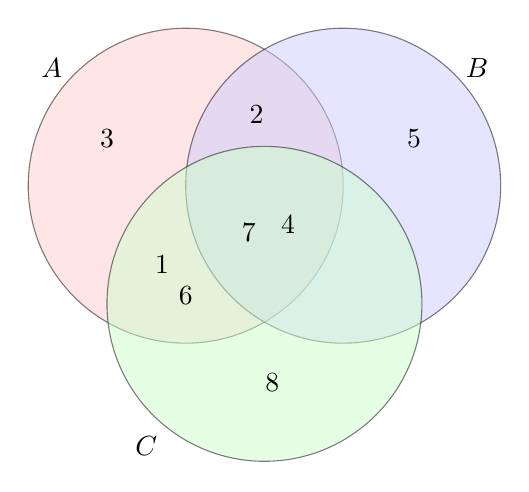
\begin{tikzpicture}
  % Draw circles
  \begin{scope}
    \fill[red!20, draw=black, opacity=0.5] (-1,0) circle (2cm);
    \fill[blue!20, draw=black, opacity=0.5] (1,0) circle (2cm);
    \fill[green!20, draw=black, opacity=0.5] (0,-1.5) circle (2cm);
  \end{scope}

  \node at (-2.7,1.5) {$A$};
  \node at (2.7,1.5) {$B$};
  \node at (-1.5,-3.3) {$C$};

  \node at (-2.0,0.6) {3};             
  \node at (1.9,0.6) {5}; 
  \node at (0.1,-2.5) {8};  
  \node at (-1.3,-1.0) {1};         
  \node at (-0.1,0.9) {2};
  \node at (0.3,-.5) {4};
  \node at (-1.0,-1.4) {6};
  \node at (-0.2,-0.6) {7};

\end{tikzpicture}

\end{document}
